\section{混和物的分离}\label{sec:4-5}

我们在生产和生活中,接触到的物质很多都是混和物,如石油、粗盐、蓝墨水等等。
化工生产的产品也常混有少量的杂质。为了适应各种不同的需要,常常要把混和物里的几种物质分开,
得到较纯净的物质,这叫做混和物的分离。这里介绍几种常用的混和物分离的方法。

\subsection{过滤}

过滤是把不溶于液体的固体物质跟液体分离的一种方法。
如粗盐的提纯就是把粗盐溶于水,经过过滤,把不溶于水的固体杂质除去。


\subsection{结晶}

\begin{wrapfigure}[13]{r}{5cm}
    \centering
    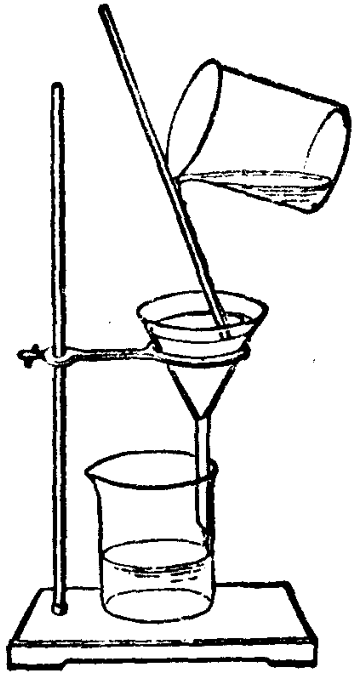
\includegraphics[width=3cm]{../pic/czhx1-ch4-9}
    \caption{过滤}\label{fig:4-9}
\end{wrapfigure}

几种可溶固态物质的混和物,可根据它们在一种溶剂里溶解度的不同,用结晶的方法,加以分离。

\begin{shiyan}
    在烧杯里加入 10 克硝酸钾和食盐的混和物(食盐的量较少)。
    注入 15 毫升水,加热,使混和物完全溶解。
    然后冷却,观察硝酸钾晶体的析出。再进行过滤(图 \ref{fig:4-9}),硝酸钾晶体留在滤纸上,
    食盐仍然溶解在滤液里。为什么?
\end{shiyan}

实验表明,先在较高的温度下制成硝酸钾的饱和溶液,由于硝酸钾的溶解度受温度的影响较大
(在 80 ℃ 时,硝酸钾的溶解度是 169 克,在 20 ℃ 时是 31.6 克),
当温度降低时,部分硝酸钾从溶液里结晶出晶体。
而食盐的溶解度受温度的影响较小
(在 80 ℃ 时食盐的溶解度是 38.4 克, 在 20 ℃ 时是 36 克),大部分食盐仍溶解在溶液里。
经过过滤,就能得到较纯净的硝酸钾晶体。但这些硝酸钾晶体仍混有少量的食盐。
大部食盐仍留在滤液里,这种滤液叫做母液。
要得到纯度更高的硝酸钾晶体,可把结晶出来的硝酸钾晶体重新溶解在蒸馏水里,加热,制成饱和溶液,
冷却,使它再一次结晶,然后过滤,食盐留在母液里。
这样的分离方法叫做\zhongdian{重结晶}或叫\zhongdian{再结晶}。
有时要经过几次结晶,才能得到纯度高的晶体。
这种分离方法能除去混和物里的杂质,得到纯净的物质,因此,又叫做提纯。结晶、重结晶在工业生产上应用很广。
例如,在化工生产上从光卤石(主要成分是 \ce{KCl . MgCl2 . 6H2O}, 还有 \ce{NaCl} 等杂质)
中分离氯化钾和氯化镁等物质;在医药工业上提纯产品等等。


\subsection{蒸馏}

蒸馏是分离和提纯液态混和物常用的方法。
应用这一方法可以把沸点不同的物质从混和物中分离出来,还可以把混在液体里的杂质去掉。
例如,在实验室里制取蒸馏水等就是用蒸馏的方法。

\begin{shiyan}
    按图 \ref{fig:4-10} 所示将蒸馏烧瓶、冷凝管、接受器等仪器装配好。
    用烧杯把混有杂质的普通水(如自来水)倒在蒸馏烧瓶里(水的体积应占烧瓶的三分之一到三分之二),
    然后用插有温度计(150 ℃)的橡皮塞把烧瓶盖紧(注意温度计的位置)。给蒸馏烧瓶加热。
    仔细观察温度的变化。当水温达到 100 ℃ 时,水沸腾,水蒸气经过冷凝管冷凝后,收集在锥形瓶里,这是蒸馏水。
\end{shiyan}

\begin{figure}[htbp]
    \centering
    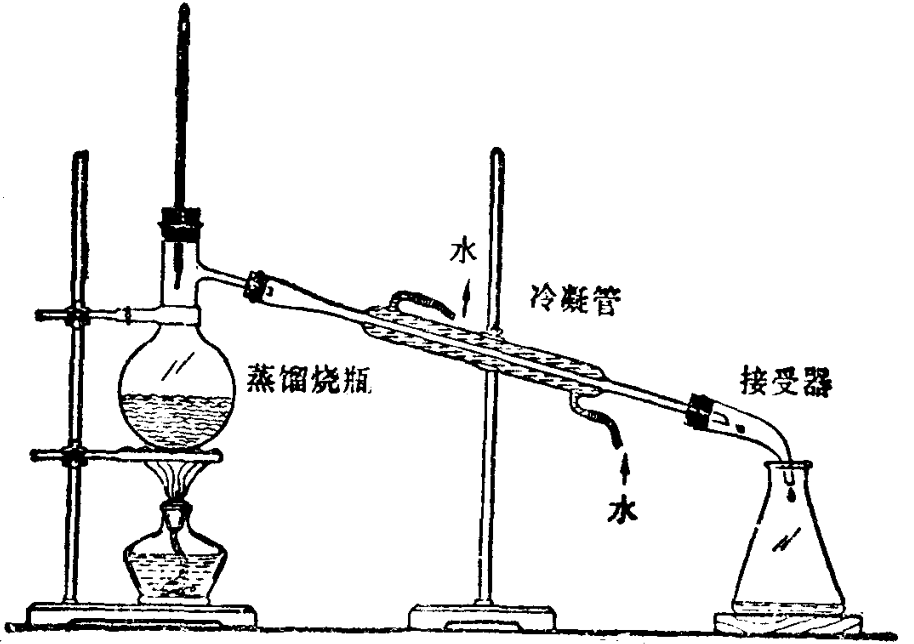
\includegraphics[width=8cm]{../pic/czhx1-ch4-10}
    \caption{蒸馏装置}\label{fig:4-10}
\end{figure}

混和物分离的方法很多,其它方法将在高中化学课里学习。


\begin{xiti}

\xiaoti{怎样从硫酸锌的溶液里把硫酸锌分离出来?}

\xiaoti{把氯酸钾和少量二氧化锰混和,放在试管里加热,使氯酸钾完全反应。在试管里剩下的物质是什么?
    写出反应的化学方程式。用什么方法可把剩下的物质分开,从而得到纯净的物质?\\
    (提示:二氧化锰不溶于水。)
}

\xiaoti{干馏和蒸馏有什么不同?}

\xiaoti{现有 30 ℃ 的硝酸钾饱和溶液 250 克。}
\begin{xiaoxiaotis}

    \xxt{当温度不变时,如果把溶剂减少 50 克,有多少克硝酸钾晶体析出?}

    \xxt{如果把 250 克饱和溶液的温度降低到 20 ℃,有多少克硝酸钾晶体析出?}

    \hspace*{2em}(提示:硝酸钾的溶解度可由表 \ref{tab:4-1} 查得。)

\end{xiaoxiaotis}

\end{xiti}

